\chapter{Literature Survey}
This literature review chapter aims to offer an in-depth review of pest control in agriculture. It begins by describing pests and emphasising their importance of pest control in crop growth. The following section discusses the causes of pest infestations, which include environmental conditions and agricultural methods. The study then delves into traditional pest management strategies and the principles of Integrated Pest Management (IPM).
The literature review then focuses on recent technology advances, and evaluates existing pest management apps. Finally, justifying the usage of Flutter for app development, highlighting the integration of Large Language Models like ChatGPT, and explaining the role of blockchain technology in securing payment systems for pesticides. This structured approach ensures a thorough understanding of pest management strategies and the tools needed for developing an innovative pest management app.

\section{Importance of Pest Control}
Effective pest control is critical for protecting crops from a variety of pests that can cause substantial damage and lower harvests. According to the report \cite{rijal_2018_farmers}, more than 80\% of vegetable producers in Chitwan, Nepal, use chemical pesticides to control pests. This dependency highlights the crucial role pest management has in agricultural yield and food security. Pests may severely harm crops, resulting in lower agricultural output and economic losses for farmers. As a result, efficient pest control is critical to guaranteeing the continuous and dependable production of crops required to fulfil the population's food demands.
\begin{itemize}
    \item Health and Environmental Concerns : While chemical pesticides are excellent pest control agents, their incorrect usage can create health issues for farmers and consumers, as well as environmental damage. A large proportion of producers are aware of pesticides' negative impacts on human health and the environment. Pesticide exposure has been linked to acute and chronic health difficulties among farmers, including skin disorders, respiratory troubles, and even more serious illnesses such as cancer. Pesticides can also pollute soil and water, having a greater ecological impact. To reduce these dangers, there is a need for improved education and training on safe pesticide usage and integrated pest management (IPM).
\end{itemize}

\section{Causes of Pest Infestations}
Pest infestations in agriculture are influenced by a variety of factors, including agricultural practices, environmental conditions, and the presence or absence of natural predators. Monoculture farming creates an ideal environment for pests, while environmental factors such as climate change and soil conditions can directly impact pest survival and reproduction. Additionally, the absence of natural predators significantly exacerbates pest problems, highlighting the need for integrated pest management strategies to maintain ecological balance and ensure effective pest control.


\subsection{Agricultural Practices} 
Monoculture refers to the agricultural practice of growing a single crop species on the same land for multiple growing seasons. This practice has become common due to its advantages, such as mechanization efficiency, improved crop varieties, and the use of chemical inputs like fertilizers and pesticides \cite{power_1987_monoculture}.
    \begin{itemize}
    \item Lack of Crop Rotation: In traditional farming practices, crop rotation was common. Different crops would be planted in succession, which would disrupt the life cycles of pests and reduce the likelihood of infestations. In monoculture, the absence of crop rotation allows pests to establish themselves more easily and multiply rapidly.
    \item Reduction in Natural Predators: Monoculture farming often leads to a decline in the population of natural predators that control pest populations. Diverse cropping systems support a wider range of species, including beneficial insects that prey on pests. In contrast, monoculture simplifies the habitat, often making it inhospitable for these natural predators.
    \item Soil Degradation: Continuous cropping without rotation can lead to soil degradation, reducing the soil's ability to support healthy plant growth. Degraded soil often results in weaker plants that are more susceptible to pest attacks. Additionally, soil erosion, which is more likely in monoculture systems, can remove nutrients from the soil, further stressing plants and making them more vulnerable to pests.
    \item Reliance on Chemical Control: Monoculture increases the reliance on chemical pesticides for pest control. While effective in the short term, this practice can lead to the development of pesticide-resistant pest populations. Over time, this can make pest infestations more severe and harder to control.
    \end{itemize}
\subsection{Environmental Factors}
Pest infestations are greatly affected by environmental variables; in this dissertation, we focus primarily on temperature, pressure, and weather patterns \cite{prasadygbambawaleom_2014_effects, skendi_2021_the}. 
\subsubsection{Temperature}
\begin{figure}[ht]
        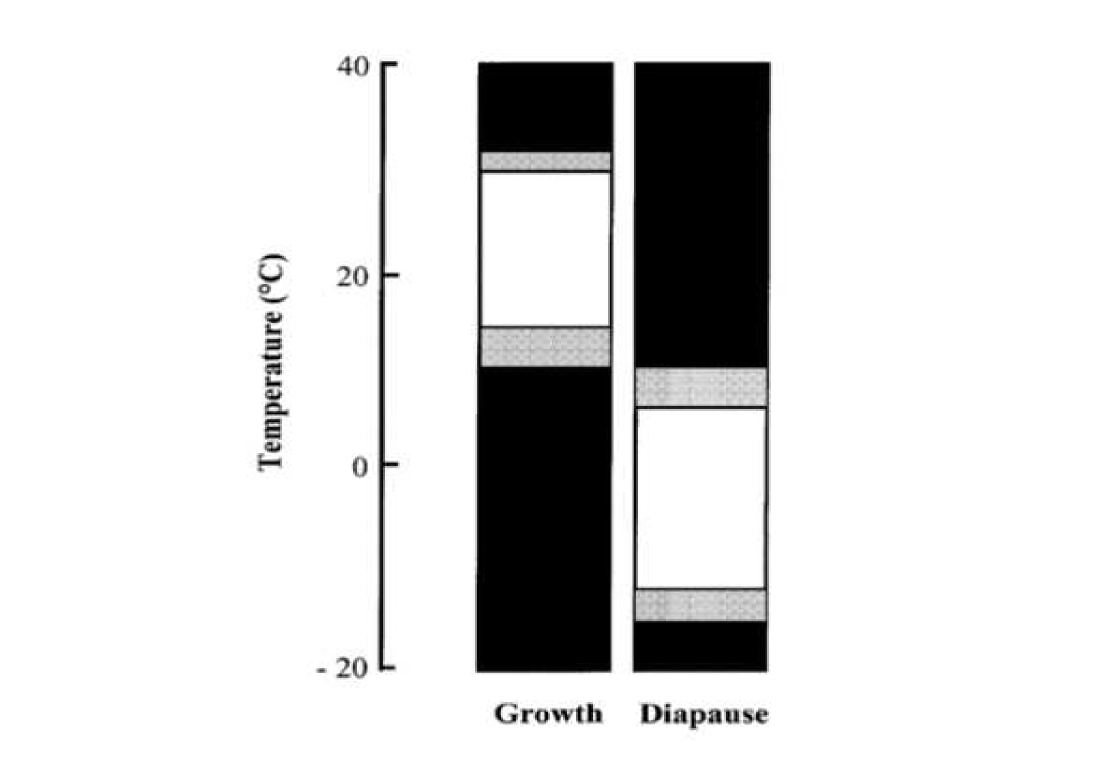
\includegraphics[width=15cm]{myReport/figures/tempature_impact.png}
        \caption{Temperature requirements for growth and diapause in
        Saturnia pavonia. Favorable temperature ranges are shown by the
        white bars, lethal temperature ranges are shown by the black bars,
        and depressing temperature ranges are shown by the grey bars.
        There is a restricted `window' for growth (white bar), with an upper and lower threshold beyond which development does not occur. To prevent imminent death when temperatures drop below c.
        5 °C, S. pavonia enters diapause; however, death follows if the temperature continues to drop. (Bebber et al., 2013)}
\end{figure}
        \begin{itemize}
        \item Acceleration of Metabolic Rates and Development: Temperature is a critical factor in the growth and reproduction of pests. Most pests are ectothermic (cold-blooded), meaning their body temperature—and thus their metabolic rate—is directly influenced by the ambient temperature. Warmer temperatures can significantly speed up the development of pests, leading to shorter life cycles. For example, pests such as the European corn borer can produce more generations per year as temperatures rise. This increase in the number of generations heightens the overall pest pressure on crops, leading to greater potential for crop damage\cite{climate2}.
        \item  Expansion of Geographical Range: As temperatures rise, the habitats suitable for many pests expand northward or to higher altitudes. Regions that were previously too cold for certain pests are now becoming viable environments for them to thrive, leading to new areas being affected by infestations\cite{climate2}.
        \item Increased Overwintering Success: Milder winter temperatures due to climate change can increase the survival rates of pests during the overwintering phase. Pests that previously would not survive harsh winters are now able to persist, resulting in larger populations emerging in the spring. This can lead to earlier and more severe infestations.
        \item Disruption of Crop-Pest Synchrony: Changes in temperature can disrupt the timing of pest emergence relative to crop growth stages. Pests may emerge earlier in the season when crops are at their most vulnerable stages, potentially leading to greater damage.
        \end{itemize}
      
\subsubsection{Humidity}
        \begin{itemize}
        \item Pest Development and Survival: Humidity plays a crucial role in the life cycle of many pests. High humidity levels can create favorable conditions for the survival and reproduction of pests, particularly those that require moist environments. For example, fungal pathogens and insects that thrive in humid conditions, such as aphids and mites, can proliferate rapidly when humidity levels are high  \cite{climate2}.
        \item  Spread of Diseases: High humidity can also promote the spread of plant diseases, which are often transmitted by insect vectors. For instance, increased humidity can enhance the survival of fungal spores or bacteria on plant surfaces, which pests can then carry to other plants, spreading disease more effectively \cite{climate2}.
        \item Influence on Pest-Predator Dynamics: Humidity can affect the interactions between pests and their natural predators or parasites. For example, high humidity may benefit pests more than their predators, leading to imbalances that allow pest populations to grow unchecked. Conversely, low humidity might reduce the effectiveness of biological control agents that require moist conditions to survive \cite{climate2}.
        \item Egg Laying and Incubation: Many pests require specific humidity levels for successful egg laying and incubation. Too low or too high humidity can reduce egg viability or delay development, impacting the population dynamics of the pest species \cite{climate2}.
        \end{itemize}
\subsubsection{Pressure}
        \begin{itemize}
        \item Influence on Pest Migration: Atmospheric pressure can influence pest migration patterns. Low-pressure systems are often associated with storm fronts, which can facilitate the movement of airborne pests, such as aphids or locusts, over long distances. This can lead to sudden and widespread outbreaks in new regions \cite{climate3}.
        \item  Changes in barometric pressure can affect the behavior of pests. For example, some insects are known to take shelter or alter their activity levels in response to dropping pressure, which often signals incoming storms. This behavioral adaptation helps them avoid being displaced by strong winds or heavy rains \cite{climate2}.
        \end{itemize}
\subsection{Absence of Natural Predators} The absence of natural predators has a significant impact on the severity and frequency of pest infestations in farms. Predatory species are critical for preserving ecological balance by putting top-down pressure on pest populations. Without these natural enemies, pests can spread uncontrolled, resulting in severe infestations and considerable economic losses. 
    However, the efficiency of natural predation in real-world settings is frequently compromised by variables such as habitat loss, agricultural practices, and pesticide usage, all of which disrupt predator habitats and reduce predator numbers and efficacy (Roy et al., 2020). The complex dynamics of predator-prey interactions, which are impacted by environmental circumstances and resource availability, make it difficult to achieve consistent pest control by natural predation \cite{roy_2020_evaluating}.


\section{Integrated Pest Management (IPM)}
Integrated Pest Management (IPM) is an agricultural method that controls pests while minimizing their impact on humans, crops, and the environment. It uses a variety of strategies to keep insect populations under control rather than depending exclusively on chemical pesticides \cite{usepa_2014_managing}. Here’s are the key components of IPM:
\begin{itemize}
    \item Monitoring and Identification: The foundation of IPM is regular monitoring of pest populations. Farmers consistently observe their fields to check for pests and beneficial organisms. This involves using traps, visual inspections, and other monitoring tools. Accurate identification of pests is crucial because different pests require different management strategies. Understanding which pests are present and in what numbers helps in making informed decisions.
    \item Setting Action Thresholds: Action thresholds are the pest population levels at which action must be taken to prevent unacceptable damage. These thresholds are based on the specific crop, pest, and local conditions. For example, a certain number of pests per plant might be acceptable, but beyond that number, intervention is necessary. Setting these thresholds helps farmers avoid unnecessary treatments, reducing costs and environmental impact.
    \item Prevention : Prevention is a critical component of IPM. Farmers use various cultural practices to prevent pests from becoming a significant problem. This includes crop rotation, which disrupts pest life cycles; planting pest-resistant varieties; adjusting planting and harvesting times to avoid peak pest periods; and maintaining field sanitation by removing crop residues and weeds that could harbor pests. These preventive measures help create an environment that is less conducive to pest buildup.
    \item Control Methods: When pest populations exceed the action thresholds, IPM employs a combination of biological, mechanical, and chemical control methods:
    \begin{itemize}
        \item Biological Control: This involves using natural predators, parasites, and pathogens to control pest populations. For example, releasing ladybugs to control aphids or using parasitic wasps to target caterpillars.
        \item Mechanical and Physical Controls: These methods include traps, barriers, and manual removal of pests. For instance, using sticky traps to catch insects or installing barriers to keep pests away from crops.
        \item Chemical Control: Chemical pesticides are used as a last resort and in a targeted manner. When necessary, selective pesticides that are less harmful to beneficial organisms and the environment are chosen. The application is based on monitoring data and thresholds to ensure minimal and precise use.
        \item Behavioral Control: Techniques such as pheromones are used to disrupt pest mating patterns or to lure pests into traps. For example, pheromone traps can be used to capture male insects, preventing them from mating with females.
    \end{itemize}
    \item Evaluation and Adaptation: Continuous evaluation is essential to determine the effectiveness of the IPM program. Farmers assess pest levels, crop health, and the economic outcomes of their actions. Based on these evaluations, they adapt their strategies to improve effectiveness. This might involve adjusting thresholds, changing control methods, or adopting new technologies.
\end{itemize}

\section{Existing Pest Management Applications}
In this section, we will look at few existing pest detection and management applications, analyse their benefits and drawbacks, and explain how they influenced the development of this dissertation project.

\subsection{Agrio - Plant health app}
\begin{figure}[ht]
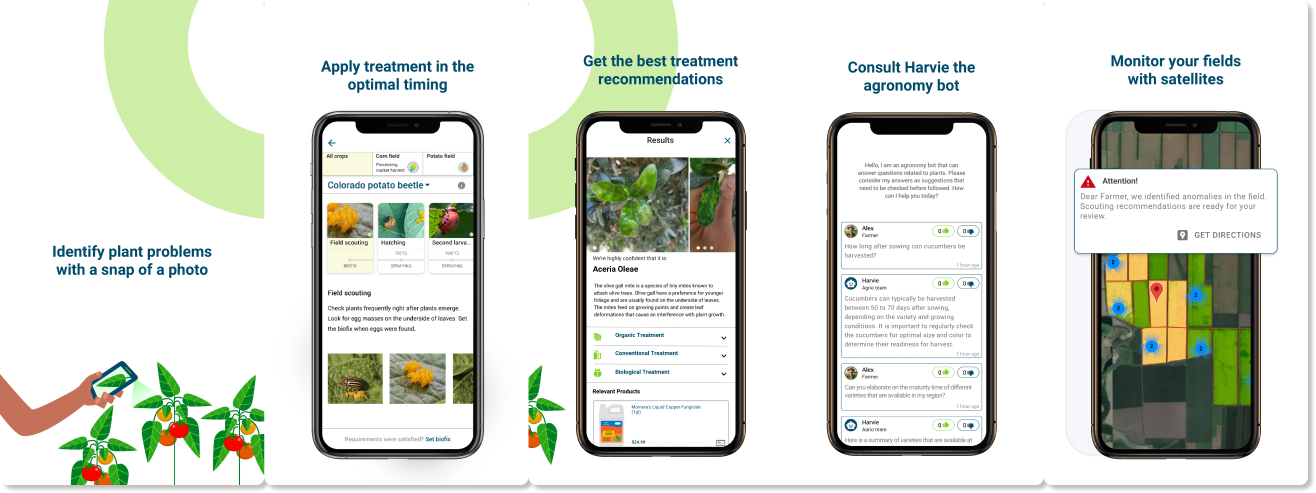
\includegraphics[width=15cm]{myReport/figures/agiro.png}
\caption{User Interface of Agrio - Plant health app}
\end{figure}
Agrio is a mobile app that helps farmers manage pests and plant diseases using advanced technology. Users can upload photos of their crops, which are analyzed by artificial intelligence (AI) to diagnose issues and recommend treatments. The app provides personalized advice through a chatbot named Harvie and supports Integrated Pest Management (IPM) by tracking pest life cycles and predicting outbreaks. Agrio includes features for collaboration, such as sharing scouting notes and creating digital reports, and uses satellite imagery for early problem detection. It also offers hyperlocal weather forecasts to help farmers anticipate potential issues and facilitates the direct purchase of recommended pesticides. While Agrio provides detailed diagnostics and useful collaborative tools, its effectiveness can be limited by the need for good smartphones and internet access, and some features require a subscription \cite{agrio_protect}.


\subsection{Advance Pesticides}
\begin{figure}[ht]
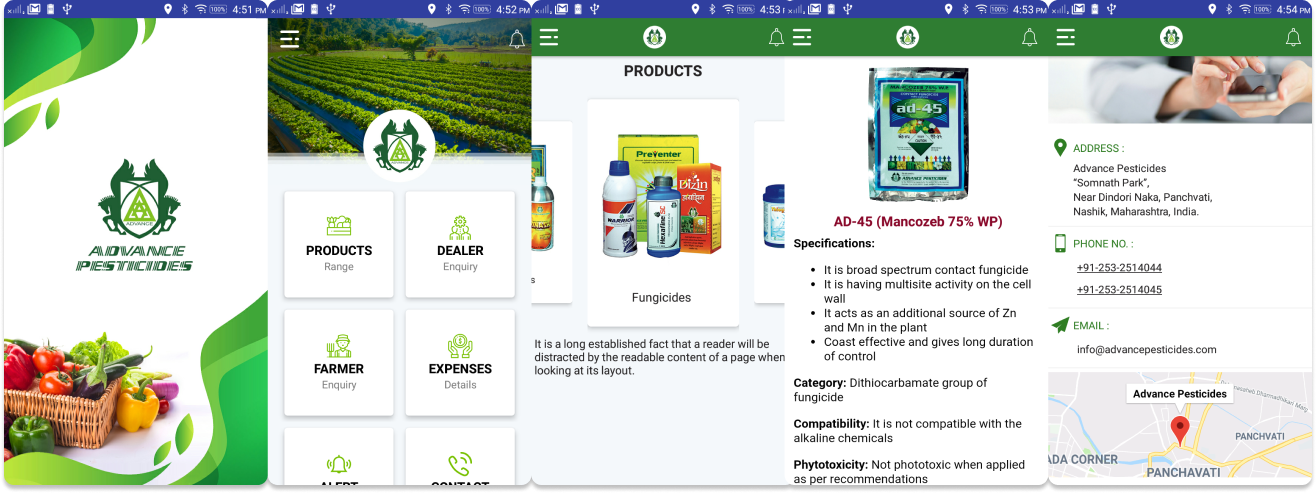
\includegraphics[width=15cm]{myReport/figures/advance_pesticides.png}
\caption{User Interface of Advance Pesticides}
\end{figure}
The Advance Pesticides app is a comprehensive tool designed to assist farmers in managing pests effectively. The app uses advanced artificial intelligence to identify pests and diseases affecting crops. Users can upload photos of their plants, and the app analyzes these images to provide a diagnosis and recommend suitable treatments. The app also offers detailed information on various pesticides, including insecticides, fungicides, and herbicides, helping farmers choose the best products for their specific needs. Additionally, the app facilitates the direct purchase of these recommended pesticides, ensuring that farmers can quickly and conveniently access the necessary products. Beyond pest management, the app includes resources for overall crop health, such as information on plant growth regulators and nutrients. This holistic approach supports farmers in maximizing their crop yield and quality while also providing educational content on safe pesticide use. Overall, the Advance Pesticides app integrates technology and convenience to enhance agricultural productivity and sustainability.



\section{Tools and Technology}

In developing the comprehensive pest management application, several cutting-edge tools and technologies are utilized to ensure a robust, efficient, and user-friendly solution. This section outlines the front-end and back-end technologies, as well as the blockchain technology used for the project.

\subsection{Front-End: Flutter}

For the front-end development, Flutter is the chosen framework. Flutter, an open-source UI software development toolkit created by Google, is the best choice for several reasons:

\begin{itemize}
    \item \textbf{Cross-Platform Development}: Flutter allows building applications for both Android and iOS from a single codebase, significantly reducing development time and costs while ensuring consistency across platforms \cite{flutter2023}.
    \item \textbf{High Performance}: Utilizing the Dart language, Flutter compiles to native code, ensuring high performance and smooth user experiences. The framework provides fast rendering and expressive UIs with its rich set of pre-designed widgets, which are crucial for creating visually appealing and responsive applications \cite{flutter_performance}.
    \item \textbf{Hot Reload}: Flutter's hot reload feature allows developers to see changes in real-time without restarting the application, accelerating the development process and facilitating UI design experimentation \cite{flutter_hot_reload}.
    \item \textbf{Rich Set of Widgets}: Flutter comes with a comprehensive library of widgets supporting Material Design and Cupertino (iOS-flavored) widgets. This enables the creation of visually appealing and functional interfaces that feel native on both platforms, enhancing user satisfaction and engagement \cite{flutter_widgets}.
\end{itemize}
Futter is an excellent choice for front-end development in this project due to its cross-platform capabilities, high performance, and rich set of widgets. Its ability to compile to native code ensures a smooth and responsive user experience across both Android and iOS platforms. The hot reload feature further accelerates the development process, making it easier to experiment with UI designs and quickly iterate on feedback. By using Flutter, the project can deliver a consistent, high-quality user experience while significantly reducing development time and cost.

\begin{figure}[ht]
        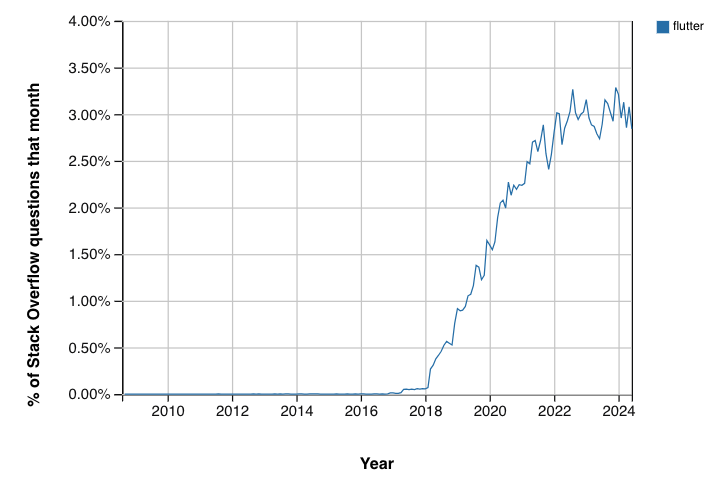
\includegraphics[width=15cm]{myReport/figures/flutter_usage.png}
        \caption{Growth of Flutter community in stack overflow (Stack Overflow Trends, 2024.)}
\end{figure}

\subsection{Back-End: Firebase}

Firebase is a popular Backend-as-a-Service (BaaS) platform, and choosing it has  several advantages, particularly since the project is cross platform mobile applications \cite{firebase}. 

\begin{itemize}
    \item \textbf{No Server Management}: Firebase abstracts away the complexities of backend server management, allowing you to focus on the frontend and core functionality of your application. This is particularly useful for a dissertation project, where time and resources might be limited.
    \item \textbf{Modular and Scalable}: Flask's modular design makes it easy to scale applications and maintain clean, organized code. Projects can be structured using blueprints, facilitating better project management and scalability. This modularity supports large-scale applications by allowing different components to be developed and managed independently.
    \item \textbf{Scalability}: Firebase is built on Google Cloud infrastructure, meaning it can scale automatically as your user base grows. This is beneficial if your dissertation project evolves into a larger application post-completion, With Firebase’s serverless model, There is no need to worry about scaling servers or managing backend infrastructure as usage increases.
    \item \textbf{Cross-Platform Support}: One of the main reason for selecting firebase as is cross platform support, Firebase supports development across multiple platforms, including web, iOS, and Android. This makes it easier to develop a cross-platform application, which could be a significant advantage.
\end{itemize}
Firebase is a highly suitable backend solution for this dissertation project, especially given the need for a scalable, cross-platform mobile application. Its serverless architecture and Google Cloud infrastructure provide automatic scalability and reliability, ensuring that the application can grow seamlessly with increased user demand. Firebase’s cross-platform support simplifies development for multiple platforms, while its abstraction of backend complexities allows for more focus on the frontend and core application features. Overall, Firebase’s features align well with the project's needs, making it a strategic choice for efficient and effective backend management.

\subsection{Blockchain Technology: Ethereum}

For secure and Payment, Ethereum blockchain technology is used. Ethereum is an excellent choice for implementing a decentralized payment system due to its capabilities:

\begin{itemize}
    \item \textbf{Smart Contracts}: Ethereum supports the creation and deployment of smart contracts, which are self-executing contracts with the terms of the agreement directly written into code. These contracts automate transactions, ensuring they are secure and tamper-proof. Smart contracts eliminate the need for intermediaries, reducing costs and increasing transaction speed \cite{ethereum_smart_contracts}.
    \item \textbf{Decentralization}: Ethereum's decentralized network eliminates the need for intermediaries, reducing transaction costs and increasing security. This decentralization ensures that payments are processed transparently and reliably, protecting against fraud and manipulation \cite{ethereum_decentralization}.
    \item \textbf{Security}: Ethereum's blockchain technology offers high levels of security, making it difficult for malicious actors to alter transaction records. This security is crucial for protecting users' financial transactions and personal information, ensuring trust in the system \cite{ethereum_security}.
    \item \textbf{Global Accessibility}: Ethereum allows payments to be made from anywhere in the world without relying on traditional banking systems, making it particularly beneficial for farmers in remote or underserved areas who may lack access to conventional financial services. This global accessibility ensures that users can participate in the economy regardless of their location \cite{ethereum_accessibility}.
\end{itemize}
Ethereum is a strong choice for implementing a secure, decentralized payment system. Its smart contracts automate transactions, reducing costs and increasing efficiency. Ethereum's decentralized network enhances security and transparency, while its global accessibility allows users to participate in the economy regardless of location, making it an ideal solution for this project.

\subsection{AI Technology: ChatGPT}

For providing detailed and accurate information on pest management, ChatGPT, a large language model developed by OpenAI, is utilized. ChatGPT is an excellent choice for this purpose due to its advanced natural language processing capabilities:\cite{ray_2023_chatgpt}

\begin{itemize}
\item \textbf{Comprehensive Information Retrieval}: ChatGPT can access and synthesize vast amounts of data to provide detailed information about various pests, including their biology, behavior, and life cycles. This comprehensive understanding is crucial for effective pest management and control .
\item \textbf{Contextual Understanding}: ChatGPT excels at understanding and responding to complex queries, allowing it to provide tailored advice on the ideal temperature, humidity, and other environmental factors for pest growth. This contextual awareness ensures that the information provided is relevant and accurate .
\item \textbf{Real-Time Decision Support}: By processing real-time data, ChatGPT can offer immediate recommendations on handling pests, including safety precautions and effective pesticide use. This capability enhances decision-making and helps in implementing timely interventions .
\item \textbf{Accessibility and Usability}: ChatGPT’s user-friendly interface and ability to generate human-like text make it accessible to a wide range of users, including those in remote or underserved areas. This ensures that critical pest management information is available to anyone, regardless of their technical expertise or location .
\end{itemize}
ChatGPT is a powerful tool for providing accurate, context-specific information on pest management. Its ability to retrieve and synthesize comprehensive data, understand context, and offer real-time support makes it an invaluable resource for this project, ensuring that users can effectively manage pests and make informed decisions. By integrating these advanced tools and technologies, the application aims to provide a seamless, efficient, and secure pest management solution for farmers. 
